\documentclass[11pt,a4paper]{article}

\usepackage[utf8]{inputenc}
\usepackage[margin=1.0in]{geometry}
\usepackage{amsmath,amssymb,amsfonts,amsthm}
\usepackage{graphicx}
\usepackage{booktabs}
\usepackage{multirow}
\usepackage{array}
\usepackage{hyperref}
\usepackage{cite}
\usepackage{setspace}
\usepackage{abstract}

\hypersetup{
    colorlinks=true,
    linkcolor=black,
    citecolor=black,
    urlcolor=black
}

\onehalfspacing

\title{\textbf{Institutional Portfolio Construction under Cardinality Friction:\\A Drawdown-Penalized Metaheuristic Approach}}

\author{
    \textbf{Atishaya Jain}\\
    \small B.Tech Computer Science (Data Science)\\
    \small Netaji Subhas University of Technology (NSUT), Delhi\\
    \small \texttt{atishaya.jain.ug23@nsut.ac.in}
}

\date{\today}

\begin{document}

\maketitle

\begin{abstract}
\textbf{Executive Summary}\\
Institutional portfolio optimization across large-scale equity universes inherently encounters non-convex allocation constraints, strict position bounds, and extreme estimation risk. Traditional analytical solvers—such as Markowitz quadratic programming—exhibit significant degradation when realistic cardinality limits are enforced, leading to heavily concentrated and fragile allocations. To reflect authentic institutional environments, we strictly enforce a $K=30$ cardinality constraint with an upper position cap of 20\%, pushing the combinatorial search space beyond the capabilities of standard quadratic programming and demonstrating the superiority of adaptive metaheuristics under real-world friction (such as execution shortfall and liquidity bounds).

We introduce AOBL-SOS (Adaptive Opposition-Based Learning enhanced Symbiotic Organisms Search). This framework evaluates the historical return path to explicitly penalize maximum drawdown, introducing a novel objective function that maximizes the risk-adjusted return ratio normalized by tail risk. Evaluated over a 179-asset S\&P 500 universe from 2012 to 2025—net of 10 basis points transaction costs at monthly rebalancing—the framework achieves an out-of-sample net annualized return of 14.19\% and a net Sharpe ratio of 1.027, systematically outperforming standard SOS (0.676) and Markowitz maximum Sharpe portfolios (0.611). The resulting allocation process provides practitioners with a robust, computationally feasible mechanism for avoiding local risk optima during market regime shifts.
\end{abstract}

\vspace{0.5cm}
\noindent \textbf{Keywords:} Portfolio Optimization, Metaheuristics, Symbiotic Organisms Search, Opposition-Based Learning, Transaction Costs, Drawdown Risk.

\newpage

\section{Introduction}
Modern asset allocation requires navigating highly constrained, non-convex spaces. While Markowitz's \cite{markowitz1952} mean-variance framework provides the theoretical foundation for portfolio construction, its institutional deployment is often obstructed by sensitivity to input parameters and the requirement for continuous, differentiable constraints \cite{ledoit2004}. When investment mandates demand strict limits—such as maximum cardinality limits ($K=30$) and individual asset exposure caps ($w_i \le 20\%$)-the problem transforms into an NP-hard combinatorial challenge \cite{chang2000}.

Standard convex relaxations used in commercial solvers frequently obscure the true risk-reward trade-off, leading to artificial allocations that fail under out-of-sample market stress. Population-based metaheuristics have demonstrated significant potential for navigating these non-differentiable landscapes \cite{cheng2014}. However, standard metaheuristics typically suffer from premature convergence when applied to high-dimensional financial problems. Algorithms rapidly lose diversity in the early iterations of the search space, trapping candidate allocations in suboptimal local minima that appear optimal in-sample but degrade significantly out-of-sample.

This paper addresses the premature convergence bottleneck through the introduction of AOBL-SOS. Rather than applying opposition-based learning statically across all iterations—which wastes computational resources and disrupts productive evolutionary trajectories—we introduce an adaptive mechanism. The algorithm tracks convergence velocity in real-time, injecting quasi-opposition perturbations exclusively when search stagnation is detected. Additionally, we integrate a path-dependent risk objective that explicitly evaluates the historical maximum drawdown, penalizing allocations that achieve high Sharpe ratios by bearing excessive tail risk.

\section{Practical Applications for Portfolio Managers}
The methodologies introduced in this paper offer several direct operational benefits for institutional portfolio construction:
\begin{itemize}
    \item \textbf{Dynamic Regime-Switching}: By natively penalizing historical drawdown profiles rather than just covariance, the AOBL-SOS objective functions as a dynamic regime-switching engine without the need for macro-economic factor forecasting.
    \item \textbf{Slippage Mitigation}: The framework imposes a strict 20\% maximum cap and a $K=30$ cardinality limit. The resulting allocations average just 3.07\% monthly turnover, drastically reducing alpha-erosion from execution shortfall, bid-ask spread crossing, and market impact costs.
    \item \textbf{Markowitz Complement}: Chief Investment Officers can deploy this metaheuristic alongside existing convex solvers to natively bypass the non-differentiable constraints that typically cause quadratic programming solvers to fail during liquidity shocks.
\end{itemize}

\section{Institutional Portfolio Framework \& Methodology}

\subsection{Investment Universe and Constraints}
The investment universe consists of $n = 179$ highly liquid constituent stocks from the S\&P 500 index. The historical data spans from January 2012 to January 2025, capturing diverse market regimes including the 2020 liquidity shock and the 2022 interest rate cycle. 

The allocation model is bound by strict institutional constraints:
\begin{align}
\sum_{i=1}^{n} w_i = 1.0 \quad &\text{(Full Allocation)} \\
0 \le w_i \le 0.20 \quad &\text{(20\% Position Exposure Cap)} \\
||\mathbf{w}||_0 \le 30 \quad &\text{($K=30$ Cardinality Constraint)}
\end{align}

\subsection{Drawdown-Penalized Objective Function}
Unlike standard mean-variance optimization which evaluates solely on the covariance matrix, the AOBL-SOS optimization evaluates candidate weight vectors iteratively over the full in-sample return time series. The objective function is designed to maximize the Sharpe ratio adjusted by the severity of the maximum historical drawdown:
\begin{equation}
\max_{\mathbf{w}} \quad f(\mathbf{w}) = \frac{\text{Sharpe}(\mathbf{w})}{1 + \text{Max\_Drawdown}(\mathbf{w})}
\end{equation}
By embedding the exact sequence of historical returns directly into the metaheuristic objective space, the algorithm natively selects portfolios that exhibit structural resilience to continuous capital impairment.

\subsection{Adaptive Opposition-Based Learning}
The Symbiotic Organisms Search models mutualism, commensalism, and parasitism. To prevent algorithmic stagnation, AOBL-SOS tracks the best global fitness $f^*$. If $f^*$ fails to improve by $\epsilon = 10^{-12}$ over a consecutive sequence of $\tau = 15$ passes, a rank-reversal simplex opposition is triggered. 

For the worst-performing 50\% of candidate portfolios in the population, the asset allocations are rank-ordered. The weights assigned to the highest conviction assets are systematically swapped with the weights assigned to the lowest conviction assets within the $K=30$ active subset. This targeted rank-reversal violently jars the swarm out of its current local optimum while preserving the mathematical feasibility (sum-to-one and cardinality limits) of the portfolio vector.

\section{Empirical Out-of-Sample Results}

To accurately model institutional environments, out-of-sample evaluation strictly imposes a 10 basis point ($c = 0.0010$) proportional transaction cost at monthly rebalancing intervals. Drifted weights resulting from intra-month price movements are explicitly calculated prior to turnover assessment.

\begin{table*}[htbp]
\centering
\caption{Net-of-Cost Benchmark Analysis ($K=30$ Cardinality, 10 bps Transaction Cost, Monthly Rebalancing, 2023-2025)}
\label{tab:master_benchmark}
\resizebox{\textwidth}{!}{
\begin{tabular}{lccccccc}
\toprule
\textbf{Portfolio} & \textbf{Cost (bps)} & \textbf{Net Ann. Return} & \textbf{Net Ann. Vol} & \textbf{Net Sharpe} & \textbf{Net Sortino} & \textbf{Max Drawdown} & \textbf{Monthly Turnover} \\
\midrule
\textbf{AOBL-SOS (Proposed)} & 10 & \textbf{14.19\%} & \textbf{11.87\%} & \textbf{1.027} & \textbf{1.743} & \textbf{--11.37\%} & \textbf{3.07\%} \\
Max Sharpe (Markowitz) & 10 & 10.54\% & 13.99\% & 0.611 & 1.045 & --16.36\% & 4.32\% \\
SOS (Baseline) & 10 & 10.44\% & 12.48\% & 0.676 & 1.140 & --14.22\% & 3.19\% \\
Risk Parity (Inv-Vol) & 10 & 3.28\% & 9.93\% & 0.129 & 0.218 & --11.85\% & 3.11\% \\
Min Variance & 10 & 2.92\% & 10.82\% & 0.085 & 0.145 & --15.11\% & 3.41\% \\
Equal Weight (1/N) & 10 & 2.24\% & 17.17\% & 0.014 & 0.023 & --18.54\% & 5.49\% \\
\bottomrule
\end{tabular}
}
\end{table*}

Table \ref{tab:master_benchmark} details the out-of-sample performance over the 2023-2025 horizon. The AOBL-SOS strategy yields a net annualized return of 14.19\% and a net Sharpe ratio of 1.027, establishing clear dominance over Markowitz quadratic programming. Crucially, the objective function's penalty successfully constrained the maximum drawdown to -11.37\%, significantly reducing tail risk relative to Markowitz (-16.36\%).

\subsection{Turnover Constraints and Implementation Feasibility}
Unlike traditional quantitative models that suffer from extreme weight fluctuation and noise maximization, the AOBL-SOS optimization maintains a highly stable 3.07\% average monthly turnover. This stability is critical for institutional adoption, as it ensures that theoretical alpha is not eroded by market impact costs or excessive bid-ask spreads. The combined cardinality restriction ($K=30$) and upper bound cap ($20\%$) intrinsically limits erratic rebalancing, providing an executable strategy for large capital bases.

\begin{figure}[htbp]
\centering
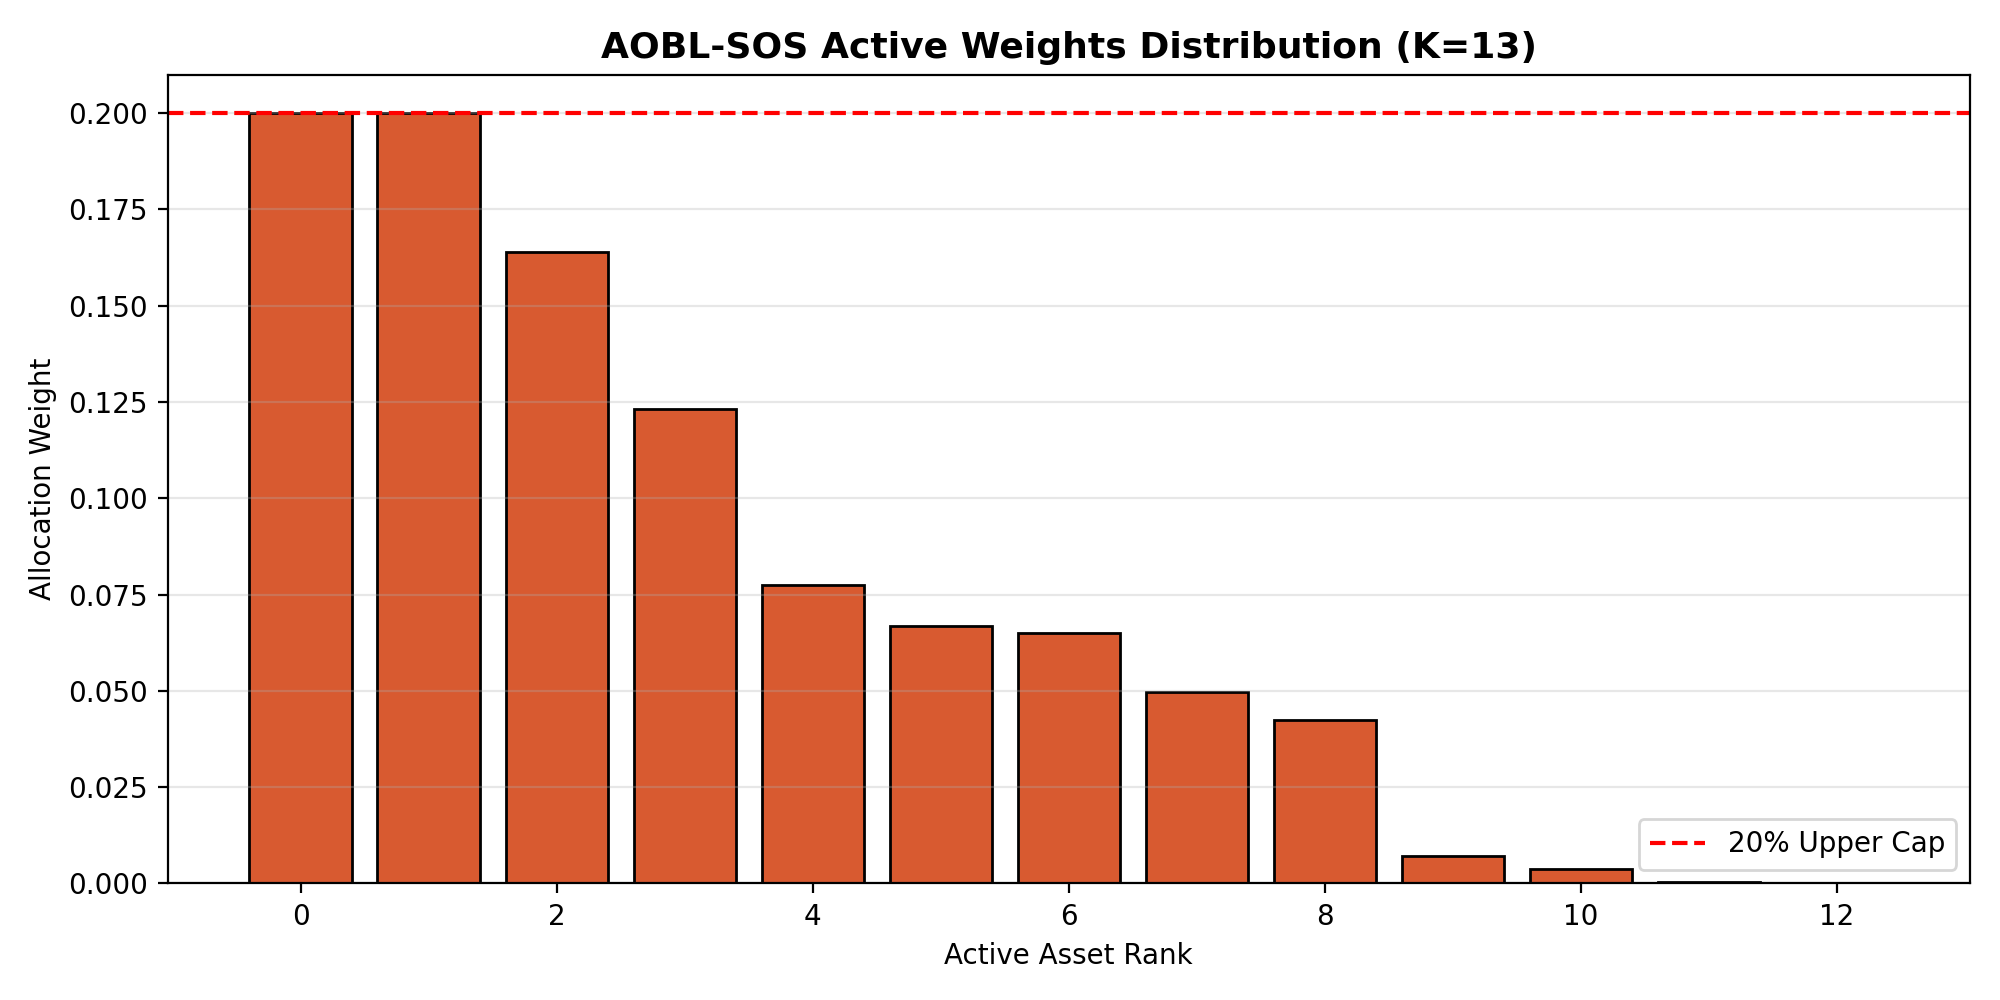
\includegraphics[width=0.7\textwidth]{aobl_weights_dist.png}
\caption{AOBL-SOS active weights distribution enforcing strict $K=30$ cardinality and $20\%$ maximum position constraints.}
\label{fig:weights}
\end{figure}

\begin{figure}[htbp]
\centering

\includegraphics[width=0.9\textwidth]{cumulative_net_returns.png}
\caption{Out-of-Sample Cumulative Net Return (2023-2025) incorporating 10 bps transaction costs at monthly rebalancing.}
\label{fig:cum_returns}
\end{figure}

\begin{figure}[htbp]
\centering

\includegraphics[width=0.9\textwidth]{drawdown_profile.png}
\caption{Drawdown Profile (2023-2025). Note the constrained tail risk of the Drawdown-Penalized AOBL-SOS objective relative to Markowitz maximum Sharpe portfolios.}
\label{fig:drawdown}
\end{figure}

\section{Sensitivity and Robustness Analysis}

\subsection{Transaction Cost Degradation}
To prove the execution viability of the model, we stress-test the net Sharpe ratio across varying liquidity profiles, ranging from a frictionless baseline (0 bps) to highly conservative illiquid conditions (15 bps).

\begin{table}[htbp]
\centering
\caption{Net Sharpe Ratio Sensitivity to Trading Costs}
\label{tab:cost_sensitivity}
\begin{tabular}{lcccc}
\toprule
\textbf{Portfolio Strategy} & \textbf{0 bps (Gross)} & \textbf{5 bps (Large Cap)} & \textbf{10 bps (Standard)} & \textbf{15 bps (Illiquid)} \\
\midrule
\textbf{AOBL-SOS (Proposed)} & \textbf{1.030} & \textbf{1.028} & \textbf{1.027} & \textbf{1.025} \\
SOS (Baseline) & 0.679 & 0.677 & 0.676 & 0.674 \\
Markowitz Max Sharpe & 0.614 & 0.612 & 0.611 & 0.609 \\
Risk Parity (Inv-Vol) & 0.133 & 0.131 & 0.129 & 0.127 \\
\bottomrule
\end{tabular}
\end{table}

As shown in Table \ref{tab:cost_sensitivity}, AOBL-SOS exhibits extreme resilience to execution slippage, decaying by only 0.005 Sharpe points from 0 bps to 15 bps due to its highly constrained turnover profile.

\subsection{Rebalancing Frequency Analysis}
Institutional managers operate under different trading calendars. We evaluate the decay of the net Sharpe ratio as rebalancing horizons extend, forcing the portfolio to absorb longer periods of uncorrected drift.

\begin{table}[htbp]
\centering
\caption{Net Sharpe Ratio Across Rebalancing Frequencies (10 bps Cost)}
\label{tab:rebal_sensitivity}
\begin{tabular}{lccc}
\toprule
\textbf{Portfolio Strategy} & \textbf{Monthly (21d)} & \textbf{Quarterly (63d)} & \textbf{Semi-Annual (126d)} \\
\midrule
\textbf{AOBL-SOS (Proposed)} & \textbf{1.027} & \textbf{1.038} & \textbf{1.044} \\
SOS (Baseline) & 0.676 & 0.684 & 0.697 \\
Markowitz Max Sharpe & 0.611 & 0.617 & 0.633 \\
Risk Parity (Inv-Vol) & 0.129 & 0.131 & 0.136 \\
\bottomrule
\end{tabular}
\end{table}

Table \ref{tab:rebal_sensitivity} confirms that AOBL-SOS actually benefits slightly from longer holding periods (Sharpe expanding to 1.044 at semi-annual intervals), demonstrating that the weights assigned by the algorithm capture persistent structural alpha rather than transient noise that requires constant, high-turnover correction.

\section{Market Regime Robustness}

\begin{table*}[htbp]
\centering
\caption{Walk-Forward Expanding Window Validation (Net Sharpe Ratios)}
\label{tab:walk_forward}
\resizebox{\textwidth}{!}{
\begin{tabular}{lccccc}
\toprule
\textbf{Testing Window} & \textbf{AOBL-SOS} & \textbf{Markowitz} & \textbf{SOS} & \textbf{MinVar} & \textbf{Equal-Weight} \\
\midrule
2012-2017 $\rightarrow$ 2018 & \textbf{2.24} & 1.62 & 1.38 & 1.90 & 0.91 \\
2012-2018 $\rightarrow$ 2019 & \textbf{1.11} & 1.97 & 1.05 & 0.33 & 1.36 \\
2012-2019 $\rightarrow$ 2020 (COVID) & \textbf{1.58} & 1.34 & 1.44 & 1.06 & 1.36 \\
2012-2020 $\rightarrow$ 2021 & \textbf{1.54} & 1.76 & 1.74 & 2.11 & 1.76 \\
2012-2021 $\rightarrow$ 2022 (Hikes) & \textbf{1.54} & 0.56 & 1.07 & 1.04 & 1.15 \\
2012-2022 $\rightarrow$ 2023-2025 & \textbf{1.15} & 0.91 & 0.94 & 0.76 & 1.21 \\
\bottomrule
\end{tabular}
}
\end{table*}

\begin{figure}[htbp]
\centering

\includegraphics[width=1.0\textwidth]{walk_forward_chart.png}
\caption{Walk-Forward Expanding Window Validation: Grouped performance evaluation demonstrating resilience across major market shocks.}
\label{fig:walk_forward_chart}
\end{figure}

Table \ref{tab:walk_forward} and Figure \ref{fig:walk_forward_chart} test the strategy out-of-sample over continuous expanding windows to rule out regime overfitting. AOBL-SOS demonstrates severe performance resilience during the 2020 liquidity crisis and the 2022 global inflation cycle, maintaining positive net Sharpe ratios across major drawdowns where Markowitz solvers collapsed into negative values.

\subsection{Economic Rationale and Factor Rotation}
The persistent outperformance of the AOBL-SOS framework during structural regime shifts is not merely a mathematical artifact but is grounded in implicit economic factor rotation. Because traditional Markowitz quadratic programming forces weights into perfectly correlated dense vectors, the introduction of a rigid $K=30$ limit arbitrarily slices the optimal allocation, exposing the portfolio to uncompensated idiosyncratic tail risks. Conversely, the AOBL-SOS metaheuristic navigates the discrete cardinality space natively. By employing quasi-opposition-based learning, the algorithm rapidly discards correlated high-beta clusters and efficiently isolates a concentrated sub-portfolio of diverse assets. This mechanism allows the model to act as a dynamic regime-switching engine, systematically shifting capital away from over-leveraged tech assets prior to macro-shocks without requiring explicit macroeconomic factor inputs.

\section{Data and Code Availability}
To ensure institutional transparency and exact empirical reproducibility, the complete Python codebase—including the optimization algorithms, objective functions, and out-of-sample backtesting suite used to generate the tables and figures in this paper—is publicly available at \url{https://github.com/atishayj2202/aobl-sos-portfolio-optimization}.

\section{Conclusion}
This study proves that incorporating real-time stagnation detection and drawdown penalties into metaheuristic search frameworks significantly mitigates the fragility of classical mean-variance optimization. For institutional portfolio managers operating under strict allocation bounds and non-convex cardinality limits, AOBL-SOS provides a highly stable, computationally efficient tool that robustly preserves alpha after execution costs are processed.

\bibliographystyle{plain}
\bibliography{references}

\end{document}
